% Source for the web edition published at isubasinghe.com/reports.
% Run `yarn build:reports` with LaTeXML installed to regenerate the HTML.
\documentclass[acmtog,screen, nonacm=true]{acmart}
\usepackage{tikz}
\usepackage{cleveref}
\usepackage{hyperref}
\usepackage{amsmath}
\usepackage{graphicx}
\usepackage{algorithm}
\usepackage[noend]{algpseudocode}

\tikzstyle{coordaxis}=[draw=red!50!black, thick, ->]
\tikzstyle{mapping}=[draw=blue!50!black, thick, ->]
\tikzstyle{connect}=[draw=green!50!black, thick, ->]



%%
%% \BibTeX command to typeset BibTeX logo in the docs
\AtBeginDocument{%
  \providecommand\BibTeX{{%
    \normalfont B\kern-0.5em{\scshape i\kern-0.25em b}\kern-0.8em\TeX}}}

\makeatletter
\let\@authorsaddresses\@empty
\makeatother

\newcommand{\floor}[1]{\left\lfloor #1 \right\rfloor}
\newcommand{\ceil}[1]{\left\lceil #1 \right\rceil}

%%
%% Submission ID.
%% Use this when submitting an article to a sponsored event. You'll
%% receive a unique submission ID from the organizers
%% of the event, and this ID should be used as the parameter to this command.
%%\acmSubmissionID{123-A56-BU3}

%%
\citestyle{acmnumeric}

%%
%% end of the preamble, start of the body of the document source.
\begin{document}

%%
%% The "title" command has an optional parameter,
%% allowing the author to define a "short title" to be used in page headers.
\title{A Distributed-Memory Simulation of the Andromeda-Milky Way Collision}

%%
%% The "author" command and its associated commands are used to define
%% the authors and their affiliations.
%% Of note is the shared affiliation of the first two authors, and the
%% "authornote" and "authornotemark" commands
%% used to denote shared contribution to the research.
\author{Isitha Subasinghe}
\affiliation{%
  \institution{University of Melbourne}
  \city{Melbourne}
  \state{Victoria}
  \country{Australia}
}
\email{isubasinghe@student.unimelb.edu.au}


%%
%% By default, the full list of authors will be used in the page
%% headers. Often, this list is too long, and will overlap
%% other information printed in the page headers. This command allows
%% the author to define a more concise list
%% of authors' names for this purpose.
\renewcommand{\shortauthors}{}

%%
%% The abstract is a short summary of the work to be presented in the
%% article.
\begin{abstract}
  In approximately 5 billion years \cite{sohn2012m31}, our Milky Way galaxy and the distant Andromeda galaxy will be merged into the Andromeda-Milky Way galaxy. We explore how a simulation of this collision could be realised through the usage of OpenMPI\footnote{See \url{https://www.open-mpi.org/}} on the Spartan HPC cloud chimera \cite{lafayette2017hpc} . The report explores how the Barnes-Hut \cite{barnes1986hierarchical} algorithm used for solving general n-body problems such as planetary body simulations could be trivially parallelised using distributed processing of the galaxies on an OpenMPI cluster. Our implementation of the Barnes-Hut algorithm over OpenMPI was able to offer a near linear speedup with respect to the number of processes used and offered a 41x speedup with 64 cores. 
\end{abstract}

%%
%% This command processes the author and affiliation and title
%% information and builds the first part of the formatted document.
\maketitle

\section{Background}
The problem of solving general n-body problems is quite simple in some sense and has arguably been known for hundreds of years following Isaac Newtons formalisation of the law of universal gravitation despite not being able to solve n-body problems in terms of integrals for n $\geq$ 3. The force exerted on an object $j$ by $i$ can be given through:
\begin{equation}
    \mathbf{F}_{j,i}=-G \frac{m_{i} m_{j}}{\left|\mathbf{r}_{ji}\right|^{2}} \hat{\mathbf{r}}_{ji}
    \label{eq:force}
\end{equation}
where: $$\mathbf{r}_{ji}=\left|\mathbf{r}_{j}-\mathbf{r}_{i}\right|$$
\vspace{1mm}
$$G \text{ is the gravitational constant}$$
\vspace{1mm}
$$\hat{\mathbf{r}}_{ji}=\frac{\mathbf{r}_{j}-\mathbf{r}_{i}}{\left|\mathbf{r}_{j}-\mathbf{r}_{i}\right|}$$
Following this understanding of basic gravitational mechanics it becomes trivial to devise an exact computational technique for solving the planetary body simulation problem. Continuing from \eqref{eq:force}, we can derive the force a set of bodies may have on object $j$ by: 

\begin{equation}
    \mathbf{F_j}=\sum_{\substack{i=0 \\ i \neq j}}^{n} -G \frac{m_{i} m_{j}}{\left|\mathbf{r}_{ji}\right|^{2}} \hat{\mathbf{r}}_{ji}
    \label{eq:allforces}
\end{equation}

And from \eqref{eq:allforces} we can finally derive the equation for updating the velocity and position of a particular body through:
\begin{equation}
    \begin{aligned}
      &\mathbf{v_{j}}^{\prime}=\mathbf{v_{j}}+\frac{\mathbf{F_j}}{m_{j}} * \Delta t \\
      &\mathbf{r_{j}}^{\prime}=\mathbf{r_{j}}+\mathbf{v_{j}} * \Delta t
    \end{aligned}
    \label{eq:posvel}
\end{equation}

We can note that the runtime complexity of solving the planetary body simulation problem through \eqref{eq:posvel} is $\mathcal{O}(n^2)$ due to the need to compare every body with every other body in the system. 
With the large number of planetary bodies in the Milky-Way alone, it becomes obvious that this naive implementation is inadequate for the task of simulating the Andromeda-Milky Way collision. It is important to note that when simulating planetary bodies of this size over such a large time-span, the act of performing the simulation accurately and in a timely manner becomes an infeasible problem, therefore making sacrifices in accuracy for increased runtime performance is an acceptable outcome. 
The Barnes-Hut \cite{barnes1986hierarchical} algorithm introduced over 35 years ago, is among one of the most commonly used algorithms for solving general n-body problems such as planetary body simulations. The algorithm offers good performance characteristics with respect to the number of bodies it simulates, however its core advantage is the relative ease of parallelising the algorithm, these properties makes the Barnes-Hut algorithm ideal for our simulation of the Andromeda-Milky Way collision. 

\section{Related Work}
The Fast Multipole Method \cite{greengard1991fast} was initially proposed to solve Gauss transforms in a performant yet accurate way but it still is capable of solving general n-body problems. The core advantage is the linear runtime $\mathcal{O}(n)$ or more accurately $\mathcal{O}(n*log(1/\epsilon))$ where $\epsilon$ is the error tolerance. As a result of the mentioned time complexity, the Fast Multipole Method benefits when there is a large number of bodies to be simulated, however it is not obvious if the real performance characteristics favour FMM and unfortunately there is no mechanical process to determine what values of $n$ favour the Fast Multipole Method over other algorithms. Blelloch \cite{blelloch1997practical} explored the various differences in the algorithms for solving the general n-body problem, they observed that the Barnes-Hut algorithm can be significantly faster when the required accuracy required is low, even for extremely large planetary body simulations. 

There have been various attempts to use the high levels of parallelism introduced in modern GPUs, some of them have been to simply perform an $\mathcal{O}(n^2)$ ``all-pairs'' calculation such as in \cite{nylons2007fast}, quite surprisingly Nyland \cite{nylons2007fast} was still able to offer a 50x speedup over the serial algorithm. Other researchers have explored as to how the Barnes-Hut algorithm could be implemented on a CUDA enabled GPU \cite{burtscher2011efficient}. Interestingly Burtscher's algorithm \cite{burtscher2011efficient} was able to offer a 74x speedup with a 240 core GPU.  

A unique, specialised approach to solving the n-body problem was proposed initially by Ito called GRAvity-PipE (GRAPE-1) \cite{ito1990special}, this approach was the development of a specialised computer (a co-processor) to perform the force calculations involved in the n-body problem, the result of using hardwired logic for the problem resulted in significant speedups. Following this initial research, there have been numerous and continuing improvements on this approach as shown by \cite{kawai2000grape, makino1997grape, makino2012grape}. 

\subsection{Parallel Algorithm}
The proposal for this idea derives from the fact that the tree building part of the Barnes-Hut algorithm is relatively simple and can be done in $\mathcal{O}(n)$ time, which is significantly faster than the $\mathcal{O}(n*log(n))$ runtime of the computation step. Initial performance testing in the development environment demonstrated that the construction step only took about 0.2\% of total computation time in the worst case. The algorithm was quite a simple variation on the sequential algorithm, we simply limited the process from calculating the force for id numbers that were not in its assigned processing range. A simple `MPI\_Allgatherv' instruction was used to broadcast the updated velocities and positions. This load balancing was quite simple to perform yet it demonstrated exceptional performance characteristics.

The parallel algorithm implemented did not make use of thread level parallelism via OpenMP \footnote{See \url{https://www.openmp.org}} and instead opted for process level parallelism through OpenMPI. The justification for this is simply as a result of our initial testing that revealed that OctTree construction time dwarfs the runtime of the actual computation time. This made it obvious that a single threaded yet multi process implementation was a viable option, especially since we could avoid NUMA and cache related performance penalties.  


\subsubsection{Integration Method}
The integration method used to solve the differential equation may have an significant effect on the accuracy of the simulation. Traditional algorithms used such as the Runge-Kutta method suffer from unbounded error. As the number of iterations of the simulation increase, it is possible that the error grows large enough such that the final result would not be an accurate simulation, this is especially important when simulating such a large time span. In order to solve this a symplectic integration technique was used called the Leapfrog method \cite{iserles1986generalized}. Leapfrog is symplectic, meaning that it is time reversible, this is an important characteristic as it means that this technique conserves the energy in the system to some bounded error. 

\subsubsection{OctTree depth}
OctTree depth has a significant impact on the runtime characteristics of the Barnes-Hut algorithm. This is ultimately as a result of how Barnes-Hut determines if an octant is worth computing exactly or not. From the algorithm for Barnes-Hut, note how $\theta$ (s/d) is calculated and checked to determine if an approximate centre of mass calculation should be used instead of an exact solution. Consider the case where we have a small maximum depth ($d_s$) to our OctTree, this means on average $s_{d_s} > s_{d_l}$ where $d_l$ indicates a larger OctTree depth, from this it is trivial to realise that $\theta_s > \theta_l$. This is an important recognition as having a smaller $\theta$ on average means that less octants will be computed exactly, leading to better performance characteristics. One more impact of the depth that we had to take into account for was the number of planets in a leaf octant, it is better for locality of reference that we have some contiguous data that we can trivially iterate over. Through experimental evaluation and taking the above considerations into account, an OctTree depth of 6 was established for the data used. 

\subsubsection{Theta Tolerance}
The tolerance level for the $\theta$ value also has a significant impact on the runtime performance of the algorithm. Consider the case where the maximum $\theta$ tolerance is capped at 0, the algorithm then simply degrades into an overly complicated $\mathcal{O}(n^2)$ ``all-pairs'' calculation. The $\theta$ value was determined through evaluation of papers such as \cite{van2013barnes} which showed that a $\theta$ value of 0.7-1.0 provided the best trade-off in terms of error and runtime.

\subsubsection{Compiler optimisations}
Compiler optimisations were heavily used to further increase the performance of the algorithm and frequent profiling of the program was done via the linux utility ``perf`` \footnote{See \url{https://perf.wiki.kernel.org/index.php/Main_Page}}. The standard library functions proved to be expensive in tight loops as a result of symbol lookup, static linking of the C++ standard library was performed in order to address this issue. Additional optimisation recommendations from \cite{fog2020optimizing} were evaluated and used where appropriate. A critical optimisation used was the ``-march=native'' flag passed onto the GNU compiler, this flag targets the exact architecture that we are compiling the program for, this results in further architecture level optimisations being possible such as usage of AVX-256.

\section{Experiments}

\subsection{Experiment Environment}
Two experimentation environments were used throughout the development process. The development environment was used as a quick way to test and filter out
ideas that weren't viable, while valid ideas were tested on the Spartan High Performance Computing cloud \cite{lafayette2017hpc}. 
\subsubsection{Development Environment}
\begin{itemize}
    \item CPU - AMD Ryzen™ 7 3700X @ 3.6-4.4GHz
    \item Memory - 32GB
    \item Compiler - GNU 11.1.0
\end{itemize}

\subsubsection{Spartan Environment}
\begin{itemize}
    \item CPU - Intel(R) Xeon(R) CPU E5-2698 v3 @ 2.30-3.6GHz
    \item Memory Per Processor - 2GB 
    \item Compiler - GNU 8.3.0
\end{itemize}




\subsection{Results}
The results were determined through running the Barnes-Hut algorithm for 30 iterations on the model B of Dubinski's work \cite{dubinski1995using} and shown below. The data does not contain every star system in the two galaxies, in fact it is a much smaller representation at just 81,920 bodies. It is important to note that this simulation starts about 1 billion years from the collision, this is largely as a result of the initial 3-4 billion years being mostly of no consequence to us. 
\begin{figure}[!h]
    \centering
    
\includegraphics[scale=0.6]{runtime.png}
    \caption{Results observed $\theta=0.7$}
    \label{fig:results}
\end{figure}

\begin{figure}[!h]
    \centering
    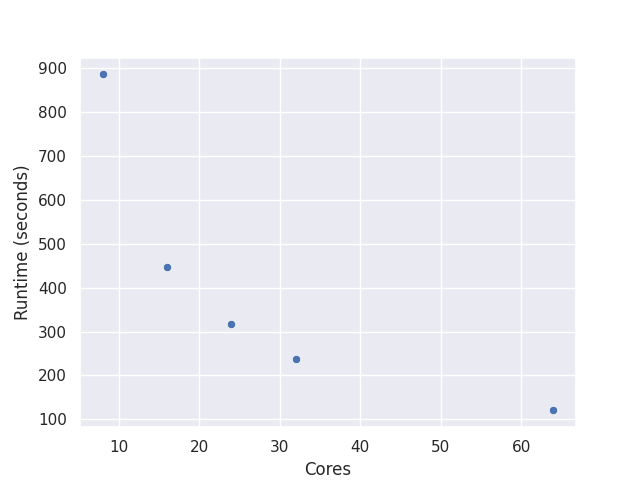
\includegraphics[scale=0.6]{runtime_theta_1.png}
    \caption{Results observed $\theta=1.0$}
    \label{fig:results_theta_1}
\end{figure}

\begin{table}[!h]
    \begin{tabular}{||c|c|c||}
        \hline
        Core(s) & $\theta=0.7$, Time(s) & $\theta=1.0$, Time(s) \\ \hline
        8   &  993.142s  & 884.421s \\ 
        \hline
        16  &  500.831s  & 446.234s \\
        \hline
        24  &  347.724s  & 318.101s \\
        \hline
        32 &   259.639s  & 237.971s \\
        \hline
        64 &   142.153s  & 120.661s \\
        \hline
    \end{tabular}
    \label{table:theta_res}
    \caption{Wall time per cores and $\theta$ value}
\end{table}
\newpage
\subsection{Discussion}
\textbf{Note: } The sequential implementation was measured to have taken 5853.931s.

Through \cref{table:theta_res} we can see that the runtimes for the algorithm are quite similar with the lower and upper bounds for our acceptable $\theta$ tolerance values that we determined earlier and therefore it makes sense to perform the full simulation with $\theta=0.7$ as it will lead to a more accurate solution despite it being slightly slower. 

An obvious limitation of our approach is the lack of accounting for the black holes at the centre of the two galaxies. When the simulation nears completion it is likely that the two black holes at the centre of both these galaxies will have a non trivial implication on how the simulation is played out. Unfortunately, no attempt was made on accounting for these gravitational effects as a result of its reliance on Einstein's theory of general relativity, while relativity can be simulated, it is much more difficult to do so than simple Newtonian mechanics. 

Unfortunately, it is likely that the 81,920 bodies approaches the largest problem size that we can simulate using this method in a timely manner, further work is required to determine how more bodies could be simulated. 

\section{Further Work}
\subsection{Simulating General Relativity}
As mentioned previously it could be beneficial to simulate Relativity instead of simple Newtonian based gravitation, solely as a result of the impacts of strong gravitation caused by the two black holes at the centre of both the Milky Way and the Andromeda galaxy. 

\section{Conclusion}
We have demonstrated how OpenMPI may be used to simulate the gravitational mechanics of large n-body problems in an effective way. As shown previously we were able to gain significant reductions in runtime performance through our distributed processing strategy. The proposed algorithm was able to offer a 41x speedup with just 64 cores, reducing a runtime of nearly 100 minutes to about 2.5 minutes, making the timely simulation of Andromeda-Milky Way collision a feasible problem. 


\bibliographystyle{ACM-Reference-Format}
\bibliography{references}

\appendix
\onecolumn
\section{Appendix}
\begin{algorithm}
\caption{Computes the new velocities and positions after one iteration of Barnes-Hut}\label{alg:naive}
\begin{algorithmic}[1]
\Procedure{RunIteration}{}
\State $\text{bodies} \gets \text{planets in the system}$
\State $root \gets \textit{OctTree root}$
\State $\text{rank} \gets \text{rank of OpenMPI process}$
\State $\text{chunkSize} \gets \text{size of chunks}$
\State $\text{size} \gets \text{number of processes}$
\State $\text{n} \gets \text{placeholder variable for number of planets}$
\State $\text{lowerBound} \gets \text{chunkSize*rank}$
\State $\text{upperBound} \gets \text{chunkSize*(rank+1)}$
\State $\text{newBodies} \gets \text{array of new bodies generated after simulation}$
\For {$i \gets 0, \ldots, n-1$}
    \If{$\text{bodies[i].id} \geq \text{lowerBound} \land \text{bodies[i].id} < \text{upperBound}$}
        \State $\text{newBody} \gets \text{simulateTimestep(root, bodies[i])}$
        \State $\text{newBodies.push(newBody)}$
    \EndIf
\EndFor
\textbf{return } \text{newBodies}
\EndProcedure
\end{algorithmic}
\end{algorithm}

\begin{algorithm}
\caption{Distributed processing of the Barnes-Hut algorithm}\label{alg:distributed}
\begin{algorithmic}[1]
\Procedure{RunDistributedBhut}{}
\State $\text{planets} \gets \text{memory of where planets are to be held}$
\State $\text{rank} \gets \text{rank of OpenMPI process}$
\State $\text{size} \gets \text{number of processes}$
\State $\text{n} \gets \text{placeholder variable for number of planets}$
\State $\text{iters} \gets \text{number of iterations to run}$
\If{$\text{rank} = 0$}
    \State $\text{planets} \gets \text{ReadPlanets()}$
    \State $\text{n} \gets \text{length(planets)}$
\EndIf
\State $\text{Broadcast(n)}$
\State $\text{Broadcast(planets)}$
\State $chunkSize \gets (n/size)+(n\%size)$
\For{$i \gets 0, \ldots, \text{iters}-1$}
    \State $\text{(origin, bounds)} \gets \text{OctTreeInitParams(planets)}$
    \State $\text{root} \gets \text{NewOctTree(planets, origin, bounds)}$
    \State $\text{localPlanets} \gets \text{RunIteration(planets, roots, chunkSize, rank, size)}$
    \State $\text{Allgather(localPlanets, planets)}$
\EndFor
\EndProcedure
\end{algorithmic}
\end{algorithm}

\end{document}
\endinput
